\documentclass[a4paper,pdftex]{article}
\usepackage{titlesec}
\usepackage{wrapfig}
\usepackage{fancyvrb}
\usepackage{amsfonts}
\usepackage{palatino}
\usepackage{lastpage}
\usepackage{color}
\usepackage{t1enc}
\usepackage[isolatin]{inputenc}
\usepackage[pdftex]{graphicx}
\usepackage{fancyhdr}
\usepackage{endnotes}
%\usepackage[pdftitle={Der Titel},pdftex=true,bookmarks=true,a4paper=true,
%           colorlinks=true,linkcolor=blue,filecolor=black,pagecolor=black,urlcolor=red, 
%            citecolor=blue]{hyperref}
             
  \lhead{\itshape \subsectionmark}
  \chead{} \rhead{\itshape Page \thepage{} of \pageref{LastPage}}
  \renewcommand{\headrulewidth}{0pt}
  \lfoot{\mbox{}\\ \itshape Radeox Developer Guide}
  \cfoot{}
  \rfoot{\mbox{}\\ \itshape  February 2004}
  
  \begin{document}
  
  \thispagestyle{empty}

  %\setcounter{page}{0}  %% Titelseite nicht mitzaehlen
  {\raggedleft\vspace{15cm}{
   \huge\bfseries\sffamily{Radeox Developer Guide}\\\vspace{0.5cm}
  \normalsize\itshape Stephan Schmidt\\
  February 2004\\\vspace{16cm}}
 
   \fbox{\parbox{\textwidth}{
   \textbf{Contact:} \\
   \begin{tabbing}
   Stephan J. Schmidt\= \quad \qquad \qquad \=
   Radeox \\
   stephan@mud.de \> \>
   http://www.radeox.org\\
   \end{tabbing}
   }}
   }
 
  \newpage
  \pagestyle{empty}
  \tableofcontents
  \newpage
  \pagestyle{fancy}
  %%\setcounter{page}{1}  %% Titelseite nicht mitzaehlen

\section{Introduction}

Radeox is a  rendering engine which renders text markup like
\_\_bold\_\_ to XHTML. Radeox uses the Java programming
language. It is used in wiki engines and 
applications  to render wiki markup. To try radeox type (you need to have commons-logging.jar in the same directory for 
this to work) into your shell or DOS prompt

\begin{verbatim}
> java -jar lib/radeox.jar
\end{verbatim}

And then at the prompt enter

\begin{verbatim}
> __radeox__
\end{verbatim}

This should render the markup to XHTML and show
\begin{verbatim}
<b class="bold">radeox</b>
\end{verbatim}

The latest version and information on how to use it can be found at http://radeox.org/.
Radeox is available under the terms and conditions of the Apache 2.0 License (see license.txt). {\it Enjoy Radeox}.

\section{Dependencies}
Radeox has the following dependencies:
\begin{itemize}
\item  commons-logging.jar
\end{itemize}
All other JAR files are needed to run the examples and the unit tests.

\section{Radeox Architecture}

Radeox uses a two stage architecture. The first stage consists of a set of filters, which
take the input and turn it into some output. 

\begin{figure}[ht]
  \centering
    
\includegraphics[keepaspectratio,width=8cm]{images/Architecture}
     \caption{\small\textsf Radeox Render Architecture}
\end{figure}

For example the BoldFilter takes as input something like

\begin{verbatim}
This is some __bold__ text. 
\end{verbatim}

and turns this into XHTML like 

\begin{verbatim}
This is some <b class="bold">bold</b> text.
\end{verbatim}

\section{Using Radeox}

All Examples can be found in the examples/ directory. The examples are wrapped
as JUnit tests and can be executed with

\begin{verbatim}
> ant test
\end{verbatim}

Using the Radeox RenderEngine in your Java applications is very simple. You just have to call render() on a RenderEngine object:

%!SRC|examples/RenderEngineExample.java|start-2|end-2|
\begin{Verbatim}[gobble=4,frame=single,numbers=left,fontsize=\small]
    RenderContext context = new BaseRenderContext();
    RenderEngine engine = new BaseRenderEngine();
    String result = engine.render("__Radeox__", context);
\end{Verbatim}
%!END

The RenderEngine needs a context object which is of Type RenderContext and contains the enviroment for the RenderEngine. RenderContext can be
implemented by yourself to pass additional parameters and enviroment variables to your filters and macros. Usually you
only use BaseRenderContext:

\begin{verbatim}
RenderContext context = new BaseRenderContext();
\end{verbatim}

That's it. Place radeox.jar into your classpath and your done.

\section{Changing input and output patterns}

\subsection{Using your own locale}

The patterns and the generated output
is not hardwired into Radeox. They can easily be changed to represent
your own wiki markup. Radeox uses locale files for the regular expression patterns and the
generated output (e.g. XHTML). These locale files have key and value pairs

\begin{verbatim}
key=value
\end{verbatim}

To adapt the mapping to your needs you have to create our yown property file
with the mappings  you want to change. All the mappings we don't want to change
are read from the standard Radeox properties locale. The standard
locale is named \textit{radeox\_markup.properties} and part of the\textit{ radeox.jar.}
Create a new file \textit{radeox\_markup\_mywiki.properties}  with the content

\begin{verbatim}
filter.bold.print=\$1<b class=\"mybold\">\$2</b>\$3
\end{verbatim}

and place the properties locale file in the classpath. Every filter
reads it's output from a property

\begin{verbatim}
filter.<name>.print 
\end{verbatim}

where 
different filters get parameters from the pattern matches.
BoldFilter gets three parameters \$1, \$2 and \$3. 
\$1 and \$3 are the matches before and after the pattern, 
\$2 is the match between the \_\_.

To change the locale the RenderEngine is using for
patterns and output, you can pass the RenderEngine an InitialRenderContext:

%!SRC|examples/RenderEngineExample.java|start-1|end-1|
\begin{Verbatim}[gobble=4,frame=single,numbers=left,fontsize=\small]
    InitialRenderContext initialContext =
        new BaseInitialRenderContext();
    initialContext.set(RenderContext.INPUT_LOCALE,
                       new Locale("mywiki", "mywiki"));
    RenderEngine engineWithContext =
      new BaseRenderEngine(initialContext);
    String result = engineWithContext.render(
        "__Radeox__",
        new BaseRenderContext());
\end{Verbatim}
%!END

The string result should now contain

\begin{verbatim}
<b class="mybold">Radeox</b>
\end{verbatim}

\subsection{Using different input and output locales}

Radeox uses different input and output locales, which can be accessed and set
in the InitialRenderContext with

\begin{verbatim}
RenderContext.OUTPUT_LOCALE
RenderContext.INPUT_LOCALE
\end{verbatim}

The input locale patterns  follow the same schema as the output locale and
are value and key pairs. The input is a regular expression pattern which is used to
find matches in the input text. The bold filter contains 

\begin{verbatim}
filter.bold.match=
    (^|>|[\\p{Punct}\\p{Space}]+)__(.*?)__([\\p{Punct}\\p{Space}]+|<|$)
\end{verbatim}

All filter keys end with {\it match} for the regular expression.
This regex can be changed to fit a different wiki markup. The OUTPUT\_LOCALE and
the INPUT\_LOCALE can be changed independently.

\subsection{Changing the properties file}

By default the locales are read from a file named {\it radeox\_markup.properties} in the
classpath. You can set the name of the file with

\begin{verbatim}
initialContext.set(
  RenderContext.INPUT_BUNDLE_NAME, 
  "myown_markup");
\end{verbatim}

Radeox then tries to load the input patterns from {\it myown\_markup.properties}. The 
name of the output properties file can be set accordingly with
      
\begin{verbatim}
initialContext.set(
  RenderContext.OUTPUT_BUNDLE_NAME, 
  "myown_markup");
\end{verbatim}

Input and output properties may be loaded from different files.

\subsection{Natural language locale}

Messages for the user which are generated by macros and filters are
read from {\it radeox\_messages.properties}. The language locale
is set with the default language locale of the JDK but can be overriden with

\begin{verbatim}
initialContext.set(
    RenderContext.LANGUAGE_LOCALE, 
    new Locale("de", "DE");
\end{verbatim}

This forces Radeox to use a German locale. To translate the macros or your own macros to
a new language, you should copy {\it radeox\_messages.properties} to
e.g.  {\it radeox\_messages\_de.properties} and then translate the values.
The locale looks like

\begin{verbatim}
#Macros
macro.table.description=Displays a table.
\end{verbatim}

The name of the messages bundle file is set with

\begin{verbatim}
initialContext.set(
    RenderContext.LANGUAGE_BUNDLE_NAME, 
    "radeox_messages")
\end{verbatim}

Another way is to inherit from BaseInitialRenderContext and create your own
InitialRenderContext where you set the appropriate values to the context. For example you can 
write a class called MyInitialRenderContext

%!SRC|examples/MyInitialRenderContext.java|start-1|end-1|
\begin{Verbatim}[gobble=0,frame=single,numbers=left,fontsize=\small]
public class MyInitialRenderContext
    extends BaseRenderContext
    implements InitialRenderContext {

  public MyInitialRenderContext() {
    Locale languageLocale = Locale.getDefault();
    Locale locale = new Locale("mywiki", "mywiki");
    set(RenderContext.INPUT_LOCALE, locale);
    set(RenderContext.OUTPUT_LOCALE, locale);
    set(RenderContext.LANGUAGE_LOCALE, languageLocale);
    set(RenderContext.INPUT_BUNDLE_NAME, "my_markup");
    set(RenderContext.OUTPUT_BUNDLE_NAME, "my_markup");
    set(RenderContext.LANGUAGE_BUNDLE_NAME, "my_messages");
  }
}
\end{Verbatim}
%!END

\section{Radeox and PicoContainer}

Sometimes it is desired to make the RenderEngine exchangeable. This can be done with a factory pattern.
But it is much more flexible to use a component container which manages the different components
of an application. There are several easy to use containers like Spring\cite{Spring} or PicoContainer\cite{PicoContainer}. The 
application puts class and interface mappings into the container and later gets the
implementation of an interface from the container without knowing which implementation
it gets. This makes it easy to change implementations of components in the application.

\subsection{Basic PicoContainer usage}

The prefered way to use Radeox is to treat the RenderEngine as a component in PicoContainer. Using Radeox this way, you
can replace the RenderEngine in Radeox easily with few changes to your code .

%!SRC|examples/PicoContainerExample.java|start-1|end-1|
\begin{Verbatim}[gobble=4,frame=single,numbers=left,fontsize=\small]
    DefaultPicoContainer dc = new DefaultPicoContainer();
    try {
      // Register BaseRenderEngine as an Implementation
      // of RenderEngine
      dc.registerComponentImplementation(
          RenderEngine.class,
          BaseRenderEngine.class);
    } catch (Exception e) {
      System.err.println("Could not register component.");
    }

    // now only work with container
    PicoContainer container = dc;

    // Only ask for RenderEngine, we automatically
    // get an available object
    // that implements RenderEngine
    RenderEngine engine = (RenderEngine)
      container.getComponentInstance(RenderEngine.class);
    RenderContext context = new BaseRenderContext();
    String result = engine.render("__SnipSnap__", context);
\end{Verbatim}
%!END

\subsection{Example with another locale}

If we want to change the locale that the RenderEngine gets at startup time, we have
to tell PicoContainer which InitialRenderContext to use. Basically the same as above, 
but we add an InitialRenderContext to the PicoContainer. PicoContainer then 
automatically configures RenderEngine with the available InitialRenderContext object.

\begin{figure}[ht]
  \centering
    
\includegraphics[keepaspectratio,width=6cm]{images/InitialRenderContextPicoContainer}
     \caption{\small\textsf InitialRenderContext in PicoContainer}
\end{figure}

%!SRC|examples/PicoContainerExample.java|start-2|end-2|
\begin{Verbatim}[gobble=4,frame=single,numbers=left,fontsize=\small]
    DefaultPicoContainer dc = new DefaultPicoContainer();
    try {
      InitialRenderContext initialContext =
          new BaseInitialRenderContext();
      initialContext.set(RenderContext.OUTPUT_LOCALE,
                         new Locale("mywiki", "mywiki"));
      dc.registerComponentInstance(InitialRenderContext.class,
                                   initialContext);
      dc.registerComponentImplementation(RenderEngine.class,
                                         BaseRenderEngine.class);
    } catch (Exception e) {
      System.err.println("Could not register component.");
    }
\end{Verbatim}
%!END

\section{Extending Radeox}

\subsection{Writing Macros}

There are several ways to extend and customize Radeox with your own ideas. 
The easiest and most powerful way to extend Radeox is to write macros. Macros
are implemented as a filter (MacroFilter). A macro in Radeox is a command that does something, 
like show the number of users,  search for a string, display a list of recently 
changed wiki pages, render source code or change the font color. 
Macros have the form \{macroname\} and can have none or several arguments.
For example \{user-count\} will display the number of registered readers in
SnipSnap.  This tutorial teaches you the basics about macros. Macros may surround content like

\begin{verbatim}
{code}
  Example code
{code}
\end{verbatim}

is rendered as

\begin{verbatim}
Example code
\end{verbatim}

\subsubsection{Macro Class}

The easiest way to write a macro is to inherit from {\it org.radeox.macro.BaseMacro}
and implement

\begin{verbatim}
public abstract void execute(Writer writer, MacroParameter params)
      throws IllegalArgumentException, IOException;
 \end{verbatim}
 
Writer is a java.io.Writer object. To output something from your macro just use

\begin{verbatim}
writer.write("hello world"); 
\end{verbatim}

If you have to output other objects than Strings then you can encapsulate
the writer with java.io.PrintWriter which supports print and println for 
several other types. Especially do not use write(i); with an int.

As an example let's write a HelloWorld macro.

%!SRC|examples/HelloWorldMacro.java|start-1|end-1|
\begin{Verbatim}[gobble=0,frame=single,numbers=left,fontsize=\small]
package examples;

import org.radeox.macro.BaseMacro;
import org.radeox.macro.parameter.MacroParameter;

import java.io.IOException;
import java.io.Writer;

public class HelloWorldMacro extends BaseMacro {
  public void execute(Writer writer, MacroParameter params)
    throws IllegalArgumentException, IOException {
    writer.write("hello world");
  }

\end{Verbatim}
%!END

This macro just writes "hello world" to the output stream. Usually it's a good idea 
to write XHTML, for example

\begin{verbatim}
writer.write("<b>Hello World</b>");
\end{verbatim}

\subsubsection{Deployment}

To make this macro run you have to first give your macro a command name. We take "hello" for this one. Add a getName method to the macro:

\begin{verbatim}
public String getName() {
    return "hello";
}
\end{verbatim}

so you can call the macro with \{hello\} from your input text. Create a jar file with two files:

\begin{verbatim}
META-INF/services/org.radeox.macro.Macro
examples/HelloWorldMacro.class
\end{verbatim}

META-INF/services/org.radeox.macro.Macro should contain lines with the class 
names of your macros, for example {\it examples.HelloWorldMacro}

Put this jar somewhere in the classpath and Radeox should find your macro.

\subsubsection{Description}

Every macro has to document itself. There is a method called getDescription. Add

\begin{verbatim}
public String getDescription() {
    return "Say hello.";
}
\end{verbatim}

to give the HelloWorldMacro a description. This description is used by 
\{list-of-macros\}.  The MacroListMacro displays all known macros 
with their name and their description.

\subsubsection{Parameters}

The execute method of Macro gets a MacroParameter object. The MacroParameter
object is created within Radeox. The RenderContext is passed from your appication 
to the MacroParameter object in your macro call.

\begin{figure}[ht]
    \centering
    
\includegraphics[keepaspectratio,width=10cm]{images/MacroParameter}
     \caption{\small\textsf MacroParameter creation}
\end{figure}

This object encapsulates useful information about the execution context. 
With params.get("0"); you can get the first un-named parameter from the macro call. To extend the macro 
to read a parameter and output the parameter after the "hello" instead of "world" rewrite execute to:

%!SRC|examples/ParameterHelloWorldMacro.java|start-1|end-1|
\begin{Verbatim}[gobble=2,frame=single,numbers=left,fontsize=\small]
  public void execute(Writer writer, MacroParameter params)
      throws IllegalArgumentException, IOException {
    if (params != null && params.getLength() == 1) {
      writer.write("Hello <b>");
      writer.write(params.get("0"));
      writer.write("</b>");
    } else {
      throw new IllegalArgumentException(
         "Number of arguments does not match");
    }
  }
\end{Verbatim}
%!END

The macro can now be used with a parameter: \{hello:Stephan\} which produces

\begin{verbatim}
Hello Stephan
\end{verbatim}

\subsubsection{Named parameters}

Arguments can be without a name, so \{image:Stephan\} displays the image with the
name "Stephan" and \{image:img=Stephan\} will do the same. 
The named version is useful when there are several optional arguments. 
If a macro is given several arguments, they are sperated with a 
"|" like in \{image:img=Stephan|align=left\}. To make the previous HelloWorld example a named
parameter, just use

\begin{verbatim}
writer.write(params.get("name"));
\end{verbatim}

which makes the macro usable as \{hello:name=Stephan\}

\subsubsection{Content block}

The content between two macro tags as in

\begin{verbatim}
{hello}
  Stephan is so funny.
{hello}
\end{verbatim}

is also part of the MacroParameter object and can be accessed with

\begin{verbatim}
params.getContent();
\end{verbatim}

This might be {\it Null} when there is no content. A ContentHelloWorldMacro could
read the name from the content and turn

\begin{verbatim}
{hello}stephan{hello}
\end{verbatim}

into 

\begin{verbatim}
hello stephan
\end{verbatim}

The code is almost the same but reads the name from the content block.

%!SRC|examples/ContentHelloWorldMacro.java|start-1|end-1|
\begin{Verbatim}[gobble=2,frame=single,numbers=left,fontsize=\small]
  public void execute(Writer writer, MacroParameter params)
    throws IllegalArgumentException, IOException {
    writer.write("hello " + params.getContent());
  }
\end{Verbatim}
%!END

\subsubsection{Reading the InitialRenderContext}

If you want to read initial parameters in your Macro you need access to the InitialRenderContext object. 
The Macro interface has a method setInitialContext which is implemented in BaseMacro like this

\begin{verbatim}
public void setInitialContext(InitialRenderContext context) {
  this.initialContext = context;
}
\end{verbatim}

The same method signature is defined in  the Filter interface. At creation time the RenderEngine implementation in Radeox calls setInitialContext on all
Macros and Filters. You can then read a value from your own InitialRenderContext. We extend the HelloWorldMacro to read the name
from the InitialRenderContext. First we have to create a InitialRenderContext and set the name as a value.

\begin{verbatim}
initialContext.set(
    "hello.name", 
    "stephan");
\end{verbatim}

The InitialRenderContextHelloWorldMacro then reads the name from the InitialRenderContext

%!SRC|examples/InitialRenderContextHelloWorldMacro.java|start-1|end-1|
\begin{Verbatim}[gobble=2,frame=single,numbers=left,fontsize=\small]
  private String name;

  public void setInitialContext(InitialRenderContext context) {
    super.setInitialContext(context);
    name = (String) context.get("hello.name");
  }

  public void execute(Writer writer, MacroParameter params)
    throws IllegalArgumentException, IOException {
    writer.write("hello "+name);
  }
\end{Verbatim}
%!END

This macro, called with \{hello\} returns 

\begin{verbatim}
hello stephan
\end{verbatim}

\subsubsection{Macros with XML closing syntax}

\subsection{Writing Filters}

While Macros are commands, filters instead replace special text markup with XHTML, for example the BoldFilter replaces \_\_bold\_\_ with <b>bold</b>. 
You should also be familiar with regular expressions\cite{Friedl} to follow this trail.

\begin{figure}[ht]
    \centering
    
\includegraphics[keepaspectratio,width=5cm]{images/Filter}
     \caption{\small\textsf Filter principle}
\end{figure}

\subsubsection{Filter Interface}

The basis for all filters is the Filter interface. All classes that want to act as filters have to implement Filter.

\begin{verbatim}
public interface Filter {
  public String filter(String input, FilterContext context);

  public String[] before();
}
\end{verbatim}

The important method is filter(). This method gets a string as an input and a FilterContext object. It takes the input string, 
applies its filtering and then returns the filtered string. FilterContext holds attributes and references, e.g. to the rendering engine.

\subsubsection{Example Filter}

To write your own filter and implement Filter there are some support classes available. The most basic is FilterSupport 
which does not much, but implement the before() method so you do not have to care. 
Most of the time though you want to use regular expressions (regex) to filter your content. 
For this there are two classes you can inherit from 

\begin{itemize}
\item RegexReplaceFilter
\item RegexTokenFilter
\end{itemize}

RegexReplaceFilter takes a regex and replaces it with some output like sed or perls s/.../.../g does. 
RegexTokenFilter calls a subroutine for every match. 

Here is a smily replace filter as an example. Suppose you want to replace every Frowny {\it :-(} with a smiley {\it :-)}. 
The only thing you have to do is to supply the regular expressions:

%!SRC|examples/SmileyFilter.java|start-1|end-1|
\begin{Verbatim}[gobble=0,frame=single,numbers=left,fontsize=\small]
public class SmileyFilter extends RegexReplaceFilter {
  public SmileyFilter() {
    super(":-\\(", ":-)");
  };
}
\end{Verbatim}
%!END

The two backslashes are for quoting the ( in the regular expression. The SmileyFilter now
replaces every occurence of \textit{:-(} in the input with \textit{:-)}. 

\subsubsection{Caching}

Radeox supports caching. To tell the engine that the output from your filter is cachable (= produces the same
output for the same input which is usually the case with static filters) add the marker interface CacheFilter
to your filter:

\begin{verbatim}
public class SmileyFilter
   extends RegexReplaceFilter 
   implements CacheFilter {
...
\end{verbatim}

You can then ask the RenderContext after a render() call, if the render result is cacheable

\begin{verbatim}
public boolean isCacheable();
\end{verbatim}

and cache the result. As a rule of thumb, if the input contained macros, the result will not be cacheable,
if it only contained filters, the result will be cacheable.

\subsubsection{Deployment}

To make this filter work you have to create a jar file with

\begin{verbatim}
META-INF/services/org.radeox.filter.Filter
examples/SmileyFilter.class
\end{verbatim}

META-INF/services/org.radeox.filter.Filter should contain lines with the class names of your filters, for example
\textit{examples.SmileyFilter}. Put this jar into the classpath and Radeox should find your filters.

\subsubsection{Using RegexTokenFilter}

Suppose we want to do something more complicated with our filter than just replace
something statically from the input. We want to write a filter which searches
for a \$ sign followed by a number in its input e.g.

\begin{verbatim}
$3
\end{verbatim}

and then replaces this with the square of the number, e.g. 9. RegexReplaceFilter fails
to do this, but luckily there is a Filter which exactly does this. RegexTokenFilter 
takes the input and splits it into tokens. For every found match, handleMatch() is called.
In the handleMatch() method you can do whatever you like with the match and
write something to the output. The SquareFilter example takes the input, converts
it to an int and returns the square.

%!SRC|examples/SquareFilter.java|start-1|end-1|
\begin{Verbatim}[gobble=0,frame=single,numbers=left,fontsize=\small]
public class SquareFilter extends RegexTokenFilter {
  public SquareFilter() {
    super("\\$[0-9]+", true);
  };

  public void handleMatch(StringBuffer buffer,
                          MatchResult result,
                          FilterContext context) {
    // group(0) will e.g. return "$3" so we have to cut the $
    int number = Integer.parseInt(
        result.group(0).substring(1));
    buffer.append(number*number);
  }
}
\end{Verbatim}
%!END

The second parameter in the super() call is whether the match is singleline or not.

\subsubsection{Using the locale versions of RegexTokenFilter and RegexReplaceFilter}

Suppose someone does not agree with your former definition of a Smiley and thinks the smiley should
look like 

\begin{verbatim}
:->
\end{verbatim}

To change the smiley he has to modify your Java code, recompile and deploy the jar. It's much easier
for him if the smiley would be defined in a properties file. Simply add the lines for a matcher and a output format
to the {\it radeox\_markup\_mywiki.properties} file (or the default Radeox properties file)

\begin{verbatim}
filter.smiley.match=:-\\(
filter.smiley.print=:->
\end{verbatim}

The standard RegexReplaceFilter does not read from a locale. While you can write the code
to read from the locale by hand, there is a helper Filter class which does this for you. LocaleRegexReplaceFilter
reads the input and output from locales. Write a LocaleSmileyFilter which extends LocaleRegexReplaceFilter:

%!SRC|examples/LocaleSmileyFilter.java|start-1|end-1|
\begin{Verbatim}[gobble=0,frame=single,numbers=left,fontsize=\small]
public class LocaleSmileyFilter
    extends LocaleRegexReplaceFilter {

  protected String getLocaleKey() {
    return "filter.smiley";
  }
}
\end{Verbatim}
%!END

The only thing you have to do is supply a key for the locale properties file. The key is then expanded to 
{\it <key>.match} and {\it <key>.print}. If you add the locale to your InitialRenderContext, the SmileyFilter should now render \textit{:-(} 
to \textit{:->}

\begin{verbatim}
InitialRenderContext context = new BaseInitialRenderContext();
Locale locale = new Locale("mywiki", "mywiki")
context.set(RenderContext.INPUT_LOCALE, locale );
context.set(RenderContext.OUTPUT_LOCALE,  locale);
\end{verbatim}

Similar to LocaleRegexReplaceFilter there is a LocaleRegexTokenFiler which reads its
parameters from the locale. This filter only reads a match key.

\section{Using Radeox in your Wiki}

\subsection{Wiki architecture}
A Wiki system usually consists of:

\begin{itemize}
\item Storage Backend (JDBC, Files)
\item Some Wiki logic to determine if a page exists
\item Some glue that takes input form the user, stores pages to the backend etc.
\item A HTML frontend, often with a web framework (WebWork, Struts, WebMacro)
\item A render engine that turns wiki markup into XHTML / XML
\end{itemize}

\begin{figure}[ht]
  \centering
    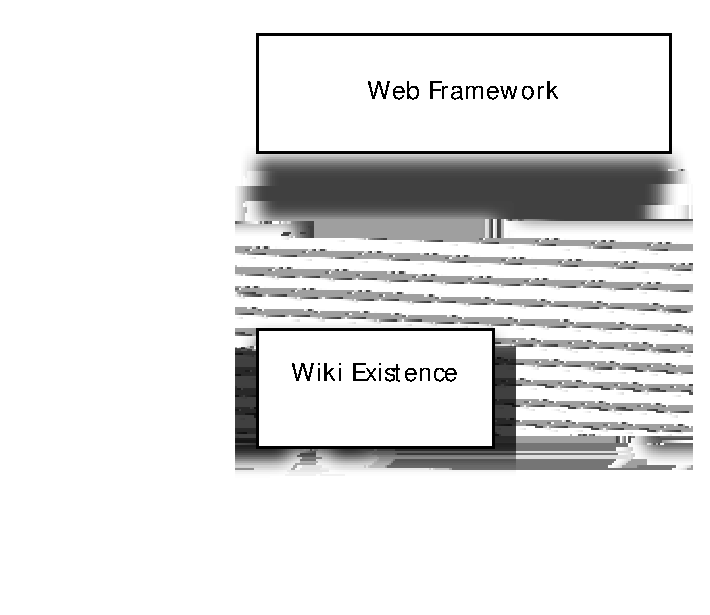
\includegraphics[keepaspectratio,width=6cm]{images/WikiArchitecture}
     \caption{\small\textsf Wiki Architecture}
\end{figure}

Although people use frameworks for the backend and the frontend, 
they mostly do not yet use a framework for the rendering engine. 
Radeox fills this gap.

\subsection{Creating wiki links}

Radeox is a wiki render engine which can be used out of the box. 
There is a render engine called BaseRenderEngine which can be used for rendering. 
This engine though does not know about you wiki backend, so you have to write your own engine. This backend
tells Radeox if a wiki page exists, if it should link to a wiki page or instead a creation form and so on.

\subsubsection{WikiRenderEngine}

For your own renderer engine you can extend BaseRenderEngine from Radeox. Then you have to implement the
interface WikiRenderEngine. This tells the renderer in Radeox that your use the renderer in a wiki enviroment and
not for another application.

\begin{verbatim}
public interface WikiRenderEngine {
  public boolean exists(String name);
  public boolean showCreate();
  public void appendLink(StringBuffer buffer, 
    String name, 
    String view, 
    String anchor);
  public void appendLink(StringBuffer buffer, 
    String name, 
    String view);
  public void appendCreateLink(StringBuffer buffer, 
    String name, 
    String view);
}
\end{verbatim}


\begin{itemize}
\item {\it exists} takes the name of a wiki page and returns true if the wiki page exists
\item {\it showCreate} returns true if radeox should render links to a creation form. This can be used to only link 'create wiki' pages if the user is logged in
\item {\it appendLink} appends e.g. the <A HREF> HTML code for linking to a wiki page with the given name to StringBuffer. View is the text that should be shown to the user.
\item {\it appendCreateLink} appends the HTML code for linking to the 'create wiki' page
\end{itemize}

\subsubsection{Making it work}

A small WikiRenderEngine, which only knows 'SnipSnap' and 'stephan' as wiki entries could look like this:

%!SRC|examples/MyWikiRenderEngine.java|start-1|end-1|
\begin{Verbatim}[gobble=0,frame=single,numbers=left,fontsize=\small]
public class MyWikiRenderEngine
    extends BaseRenderEngine
    implements WikiRenderEngine {

  public boolean exists(String name) {
    // make a lookup in your wiki if the page exists
    return name.equals("SnipSnap") || name.equals("stephan");
  }

  public boolean showCreate() {
    // we always want to show a create link, not only e.g.
    // if a user is registered
    return true;
  }

  public void appendLink(StringBuffer buffer,
                         String name,
                         String view) {
    buffer.append("<a href=\"/show?wiki=");
    buffer.append(name);
    buffer.append("\">");
    buffer.append(view);
    buffer.append("</a>");
  }

  public void appendLink(StringBuffer buffer,
                         String name,
                         String view,
                         String anchor) {
    buffer.append("<a href=\"/show?wiki=");
    buffer.append(name);
    buffer.append("#");
    buffer.append(anchor);
    buffer.append("\">");
    buffer.append(view);
    buffer.append("</a>");
  }

  public void appendCreateLink(StringBuffer buffer,
                               String name,
                               String view) {
    buffer.append(name);
    buffer.append("<a href=\"/create?wiki=");
    buffer.append(name);
    buffer.append("\">");
    buffer.append("?</a>");
  }

  public String getName() {
    return "my-wiki";
  }
}
\end{Verbatim}
%!END

Then use the render engine as described before. You have to set your engine in BaseRenderContext though, 
so Radeox does use your engine to determine if wiki pages exist. The LinkFilter in Radeox 
takes a look at your RenderEngine and if it implements WikiRenderEngine, Radeox uses your WikiRenderEngine
to look for existing wiki pages and for creating XHTML links.

\begin{verbatim}
RenderEngine myEngine = new MyWikiRenderEngine();
RenderContext context = new BaseRenderContext();
context.setRenderEngine(myEngine);
String result = myEngine.render("My String", context);
\end{verbatim}

Alternativly  you could create your own RenderContext that returns your engine. That's it.

\subsection{Changing the linking style to WikiLinkingStyle}

\subsection{Porting to Radeox}

For example, WikiLand uses Cocoon for rendering. To change their architecture
to use Radeox they would have to insert the Radeox API between their application
and their wiki markup renderer. 

\begin{figure}[ht]
  \centering
    
\includegraphics[keepaspectratio,width=10cm]{images/WikiLand}
     \caption{\small\textsf WikiLand and Radeox integration}
\end{figure}


\section{Writing your own RenderEngine}

You want to write a completely different RenderEngine for 
Radeox (or SnipSnap). Perhaps you want to render XML to XHML 
using XSLT or you want to support other wiki markup and your goal 
cannot be achived with writing macros or filters.
Perhaps you want to use a parser instead of regular expressions.

\subsection{Write a Radeox RenderEngine}

The RenderEngine interface looks like this:

\begin{verbatim}
public interface RenderEngine {
  public String getName();
  public String render(String content, RenderContext context);
}
\end{verbatim}

You write your own Implementation of RenderEngine, 
say MyRenderEngine where getName() returns "my" and 

\begin{verbatim}
render(content, context);
\end{verbatim}

does the actual rendering, for example replace all "X" with "Y":

%!SRC|examples/MyRenderEngine.java|start-1|end-1|
\begin{Verbatim}[gobble=0,frame=single,numbers=left,fontsize=\small]
public class MyRenderEngine implements RenderEngine {
  public String getName() {
     return "my";
  }
  public String render(String content, RenderContext context) {
     return content.replace('X', 'Y'); 
  }
\end{Verbatim}
%!END

\section{Using Radeox from other languages}

\subsection{Writing Macros with Groovy}

Groovy\cite{Groovy} is a scripting language which directly 
compiles to byte code for the Java VM. There are two ways to use
Groovy with Radeox

\begin{itemize}
\item compiling Macros to .class files
\item loading Groovy Macros from Java
\end{itemize}

%!SRC|examples/GroovyMacro.groovy|start-1|end-1|
\begin{Verbatim}[gobble=0,frame=single,numbers=left,fontsize=\small]
package examples;

import java.io.Writer
import org.radeox.macro.parameter.MacroParameter

class GroovyMacro extends org.radeox.macro.BaseMacro {
  void execute(Writer writer, MacroParameter params) { 
    writer.write("Yipee ay ey, schweinebacke")
  }
  String getName() {
    return "groovy"
  }
}
\end{Verbatim}
%!END

You can use ant to compile the Groovy Macro to Java code. It's easier first compile 
all Groovy scripts to a destination directory and after that your Java files, because
otherwise the Java compiler won't find the Groovy .class files.

\begin{verbatim}
<target name="compile-groovy" depends="prepare">
  <groovyc destdir="${pre-out}" srcdir="${src}" listfiles="true">
      <classpath refid="classpath"/>
  </groovyc>
</target>

<target name="compile" depends="prepare, compile-groovy">
  <javac srcdir="${src}" destdir="${out}" classpathref="classpath"/>
</target>
\end{verbatim}

The {\it pre-out} directory is in the classpath, so the javac task finds the compiled Groovy 
files. See the build.xml in the examples directory for a working example. To make the
groovyc task working, you jave to first add

\begin{verbatim}
  <taskdef name="groovyc" classname="org.codehaus.groovy.ant.Groovyc" classpathref="classpath"/> 
\end{verbatim}

to your build.xml

\subsubsection{Loading Macros with Groovy at runtime}
A Java class which compiles this macro source code to a Macro is GroovyMacroCompiler

%!SRC|examples/GroovyMacroCompiler.java|start-1|end-1|
\begin{Verbatim}[gobble=0,frame=single,numbers=left,fontsize=\small]
public class GroovyMacroCompiler  {
 public Macro compileMacro(String macroSource) {
    Macro macro = null;
    try {
      GroovyClassLoader gcl = new GroovyClassLoader();
      InputStream is = new ByteArrayInputStream(
          macroSource.getBytes());
      Class clazz = gcl.parseClass(is, "Macro.groovy");
      Object aScript = clazz.newInstance();
      macro = (Macro) aScript;
    } catch (Exception e) {
      System.err.println("Cannot compile groovy macro.");
    }
    return macro;
  }
}
\end{Verbatim}
%!END

\begin{thebibliography}{}
\bibitem{Groovy} Groovy programming language, http://groovy.codehaus.org
\bibitem{PicoContainer} Component container, http://www.picocontainer.org/
\bibitem{Spring} Spring Framework with component container, http://www.springframework.org/
\bibitem{Friedl} Jeffrey E. F. Friedl, Mastering Regular Expressions, ISBN: 0596002890
\end{thebibliography}
\end{document}
